\documentclass[12pt,a4paper]{article}

%%%% Includes

\usepackage[utf8]{inputenc}

\usepackage{color}

\usepackage{wrapfig} % text wrapping figures
\usepackage{subcaption}

\usepackage{graphicx} % images

\usepackage{setspace}

\usepackage{hyperref}

\usepackage{etoolbox}
\patchcmd{\thebibliography}{\section*{\refname}}{}{}{}

\onehalfspacing


%%%% general information %%%%
\title{browser fingerprinting for Learning Analytics}
\author{Luis Glaser}
\date{2018 \\ March \\ 20}

\begin{document}

%%%%%%%%%%%%%%%%%%% TITLEPAGE BEGIN %%%%%%%%%%%%%%%%%%%
\begin{titlepage}
\centering
    {\scshape\LARGE Institut für Informatik\par}
    {\scshape\Large Goethe Universität Frankfurt am Main\par}
    \vspace{2cm}
    {\huge\bfseries Device Fingerprinting for Learning Analytics\par}
    \vspace{2cm}
    {\Large\itshape Seminararbeit zu Computational Humanities - Learning Analytics\par}
    {\large Prof. Dr. Hendrik Drachsler\par}
    \vfill
	
    {\large \today\par}
    \vspace{1.5cm}

% Bottom of the page
    Luis Glaser\par
    Martikelnummer: 5312890\par
    Informatik B.Sc.\par
\end{titlepage}
%%%%%%%%%%%%%%%%%%% TITLEPAGE END %%%%%%%%%%%%%%%%%%%

\pagenumbering{gobble}

\tableofcontents
\pagebreak
\pagenumbering{arabic}
% !TEX root = ../main.tex
\label{sec:abstract}

\begin{abstract}
\emph{Abstract} - Education is being reinforced by technology more and more from which students and teachers alike can profit. Even when students are part of or enrolled in one institution, the educational content they consume will most likely be distributed across the web. To improve the quality of a course, these resources should be taken into account as well, e.g. via suggestions to other students. In order to incorporate these sources without relying on traditional ways of identification like user accounts or cookies, browser fingerprinting can be a valuable alternative.

This work examines the recent work that has been done on web fingerprinting technology. Also, their effectiveness and limitations are discussed. Additionally, some of the available fingerprinting technology will be demonstrated and tested in a student-grade webservice. Finally, we envision a possible integration scenario for Learning Analytics.  
\end{abstract}

% section introduction (end)
% !TEX root = ../main.tex
\section{Introduction} % (fold)
\label{sec:introduction}

With the advent of online learning platforms like moodle a way to centralize the learning experience for students has come up. Students are able to perform tasks, upload their exercises or consume additional study material on web platforms that might be offered by their school or university. 
But not only material that is being dedicatedly distributed by an institution is also used for learning by students. Many students use external material. This might be used for deepening their understanding of the current topic or seeking additional aid for exercising. This again limits the ability of a tutor or teacher to monitor their students' activities.

Furthermore, Recommendation Systems play a central role in Technology Enhanced Learning Environments. As soon as the recommendation is based in some way on what peers or other students in general have used to study, another problem arises: 
There needs to be some way to collect data on who is viewing what content, maybe even enriched by quality or satisfaction measures \cite{ricci_panorama_2015}. This might be feasible when the content in question is held by one provider only, but becomes increasingly harder, when students are using external content, be it online video tutorials or \textit{MOOCs}. Despite being material from external sources, they might provide additional value to a students curriculum. 

In order to also incorporate these external materials into a learning platform or a recommendation system, their usage by a student needs to be tracked in someway. This might still be possible when using in-house technology, but will be made increasingly harder when students are using their private devices. 

One approach from the content providers side would be, to track their visitors and then associate them with the student that is using a Technology Enhanced Learning Environment in question. This would hold multiple benefits: \begin{itemize}
\item (1) No form of user account would be necessary, which could broaden the scope of used learning material beyond usual hubs users often have user accounts with.
\item (2) Is ideally independent from a users device, \cite{yen_host_2012,cao_cross-browser_2017,acar_web_2014} which makes it lightweight for a user and sustainable for a learning platform. 
\end{itemize}

This opens the topic of this paper, accessing the usage of fingerprinting in the field of Learning Analytics. The main focus will be on recent research on fingerprinting while keeping the education focused usage scenario in mind.

The paper will be structured as follows. Section \ref{sec:sota} will first give an explanation on what fingerprinting does and how we can use it. Section \ref{subsec:fpatt} will enumerate and discuss possible and combinable ways to fingerprint a given browser, while keeping resource efficiency in mind. We then propose criteria what such a fingerprinting tool should offer and present a tool that has been used to fingerprint browsers in Section \ref{sec:method}. Section \ref{sec:results} will then discuss the results of the research undertaken and suggest a few ways of improvement. Section \ref{sec:conclusion} will then conclude.
 
% !TEX root = ../main.tex
\section{State of the Art} % (fold)
\label{sec:sota}



\subsection{Browser Fingerprinting}

%% Definition of fingerprint
In this paper the term \textit{fingerprint}, if not specified further, will refer to a \textit{browser fingerprint} analogously to the suggestion by Acar and colleagues: ``A [browser] \textit{fingerprint} is a set of system attributes that, for each [browser], take a combination of values that is, with high likelihood, unique, and can thus function as a [browser] identifier.'' \cite{acar_fpdetective_2013}. It should thus be noted, that most of the features that will be discussed in section \ref{subsec:fpatt} will focus on \textit{browser fingerprinting}. Features like the \texttt{User-Agent} String or most of the features extracted via JavaScript can differ from browser to browser. Fingerprinting across different browsers on one machine introduce another level of complexity. Then, multiple \textit{browser fingerprints} need to be merged into one \textit{device fingerprint} \cite{cao_cross-browser_2017}.

As already hinted, browser attributes can add different levels of value for fingerprinting. Some attributes may have only a limited number of states or be shared between many devices (e.g. boolean variables or coarse OS version). Other attributes contribute a lot to the quality of a fingerprint like the list of fonts \cite{acar_fpdetective_2013,laperdrix_beauty_2016}. Thus, the likelihood of uniqueness does not only increase by the number of values we extract, but also by the quality of those values. 

Some of these areas from which browser attributes can be extracted are rather new, like the \texttt{WebGL API} and all features of the \texttt{HTML5 canvas} element. Others are on the way to be phased out like \texttt{Flash}, \texttt{Silverlight} or in-browser \texttt{Java}, as Laperdrix and colleagues have already seen in their dataset \cite{laperdrix_beauty_2016}.

Research about web fingerprinting does not only focus on how values to differentiate are generated, but also how other identifiers can be persistently saved. Acar and colleagues have pointed out that content providers use cookie syncing to further keep alive a cookie, even after users have cleared their cookies and cache \cite{acar_web_2014}. This technique might be valuable when applying it to Learning Analytics since it could be used to preserve a students history within restricted environments like computer labs and others.

The possibilities and limits of fingerprinting have found recent attention in research. Their work has been focused on three main areas. (1) Discovery of new attributes that can be used to fingerprint \cite{murdoch_hot_2006,mowery_pixel_2012,fifield_fingerprinting_2015}, (2) studies that try to test the effectiveness of browser fingerprinting \cite{laperdrix_beauty_2016,eckersley_how_2010,nikiforakis_cookieless_2013} and (3) find ways to detect websites that employ someway of fingerprinting \cite{nikiforakis_cookieless_2013,acar_fpdetective_2013,acar_web_2014}. 
For the purpose of this research, we will mainly address studies from (1) and (2). (3) will be useful to us for looking at how the industry already uses this technology and what we can learn from that when transferring to Learning Analytics.

\subsection{Fingerprintable Attributes}
\label{subsec:fpatt}

In this section we will discuss different fingerprinting attributes, how we can obtain them and their quality if they have been tested already.

It must be noted, that the enumeration in Table \ref{fptable} is not exhaustive, it only contains attributes that have either been mentioned in multiple papers or that have been empirically studied in at least one. Eckersley also mentions fingerprinting irregularities within the TCP/IP stack, clock skew and others \cite{eckersley_how_2010}.
The available fingerprinting techniques presented below are not exclusive to each other but are most valuable when combined in order to increase the quality of a browsers fingerprint.
%%
\subsubsection{HTTP-Header}
\label{sota:httpheader}
The most straightforward source of fingerprintable attributes is the \texttt{HTTP\-Header}. It's being sent with every request and response message and can thus be obtained fairly easily. A variety of them is context-dependent, like the \texttt{referer} field, which thus are not useful for fingerprinting. The permanent ones have already been exploited by a few studies \cite{laperdrix_beauty_2016,eckersley_how_2010} and proven to contribute significantly to the diversity of fingerprints.\footnote{Shannon's entropy for the AmIUnique dataset was $0.570$, $0.531$ for the Panopticlick dataset \cite{laperdrix_beauty_2016}.} 

The \texttt{HTTP-Header} becomes even more important on mobile devices, since applications and even mobile carriers are customizing the \texttt{User-Agent} Attribute of the \texttt{HTTP-Header} which increases the likelihood of discriminating information\cite{laperdrix_beauty_2016}. Some browser extensions offer spoofing of the \texttt{User-Agent} String. This, counterintuitively, makes the browser more distinguishable because unless many other browser share this spoofed string, the group they share the string with is smaller then a basic wide spread \texttt{User-Agent} string \cite{eckersley_how_2010}.


\subsubsection{Fonts}
\label{sota:fonts}
Fingerprinting characteristics in browsers based on their displayed font can be carried out in two ways. Either by (1) fingerprinting the set of available fonts of a browser and secondly by fingerprinting the (2) rendering process of single symbols of a font

(1) The variety of fonts installed on a device can be very revealing as found by Laperdrix and colleagues \cite{laperdrix_beauty_2016}. These can either be revealed directly via browser plug-ins like Flash or Java. When collecting the list of fonts from these sources they are unordered thus adding additional entropy by the order they are returned in \cite{nikiforakis_cookieless_2013}. Modern privacy oriented browsers already block these types of direct enumeration of fonts \cite{fifield_fingerprinting_2015}. These can be bypassed by rendering a string of a given font, measuring its dimensions and comparing them to a fall-back font named \texttt{"Non-Existent-Font"} or something similar. If the dimensions differ, the font is available in the browser. Furthermore, Font Fingerprinting is even more revealing on mobile devices since many manufacturers on Android offer their own designs, thus enabling fingerprinting down to device level \cite{acar_fpdetective_2013}.

The more browser centered approach targets the rendering of font directly. (2) This renders single glyphs from Unicode and compares the hashes. Unlike the previous variant fonts aren't targeted directly but called by general \texttt{CSS}-names like \texttt{sans-serif} or \texttt{cursive}. This discloses both browser specific design choices and device particularities of the OS font rendering engine. \cite{fifield_fingerprinting_2015}

Of course, all these processes are performed off the screen and is thus transparent to the user. Fifield and Egelman have found the latter technique to be more discriminating then the \texttt{User-Agent}. Their font metric measured $1.5$ times the entropy of the \texttt{User-Agent} string \cite{fifield_fingerprinting_2015} .

\subsubsection{Canvas}
\label{sota:canvas}
\cite{mowery_pixel_2012} Canvas fingerprinting is only little more complex than font fingerprinting but is able to add further diversity to a fingerprint. Introduced with \texttt{HTML5}, the \texttt{canvas}-Object enables tighter interaction with a device's underling hardware. Intended for enabling more sophisticated Web Applications, this can also be used to extract quirks not only from browser implementations but also from a device's hardware \cite{mowery_pixel_2012}. The fingerprinting works by drawing forms or text on this canvas object and then collecting the hashed return values from \texttt{toDataURL(type)}. Since only the hashed value ends up in the fingerprint, this can also be performed rather easily. 
Mowery and Shacham have also suggested drawing 3D forms onto a \texttt{canvas} to add more complexity, but Laperdrix and colleagues found these to be non consistent \cite{laperdrix_beauty_2016}.\footnote{resizing the browser window and redoing the test returned other values.} However, it's consistent and viable for drawing 2D forms, fonts or extracting values like the GPU vendor or make.

\subsection{Further possibilities for fingerprinting}
\label{subsec:furtherposs}

This section will point out additional elements that can be fingerprinted but have either not been studied extensively yet or not in the connection to fingerprintability. However they need to be pointed out, in case the intended use case in Learning Analytics especially profits from one or more of them.

Another way to find unique features of a browser is not within the realm of values but more in the realm of attributes themselves. Browser functionality today is relatively standardized, but the implementations still offer some unique features which can be fingerprinted as well, for example the \texttt{screen.\underline{moz}Brightness} in Mozilla Firefox or \texttt{navigator.\underline{ms}DoNotTrack} in Internet Explorer \cite{nikiforakis_cookieless_2013}.

Also, the viability of fingerprinting characteristics are different between mobile and desktop devices. As there are no plug-ins or \texttt{Flash} on mobile devices, the bulk part of diverseness must come from other values as the User-Agent.\footnote{Phone Carriers include their name in addition phone model and other information in the \texttt{User-Agent}.}\cite{laperdrix_beauty_2016}.

% !TEX root = ../main.tex
\section{Method} % (fold)
\label{sec:method}

After having reviewed recent research on fingerprinting, we turn to test the technique. Unfortunately due to the limited scope of this seminar paper we will focus on a small scale example fingerprinting of the aforementioned \texttt{HTTP-Header} values. 

\subsection{User recognition}
\label{subsec:userrecognition}
To test the described fingerprinting method, we create a small online fingerprinting service. In a live scenario, we will depend on recognizing revisiting users to leverage this service properly. When seeing User $U$, represented by his browser, having $n$ fingerprints $f_1, f_2, \ldots, f_n$ in our database, several things can occur:

\begin{itemize}
	\item $(1)$ (\emph{True Positive}): $U$ has visited already and we \textit{correctly} connect him to Fingerprint $f_U$.
	\item $(2)$ (\emph{False Positive}): $U$ has not visited yet and we \textit{falsely} connect him to Fingerprint $f_V$ or create a new one.
	\item $(3)$ (\emph{False Negative}): $U$ has visited already but we \textit{falsely} do not connect her with the correct $f_U$, instead creating a new one.
	\item $(4)$ (\emph{True Negative}): $U$ has not visited yet and we \textit{correctly} connect her to a new Fingerprint $f_U$.
	\label{item:cases}
\end{itemize}

\begin{wrapfigure}{r}{0.5\textwidth}
\centering
\frame{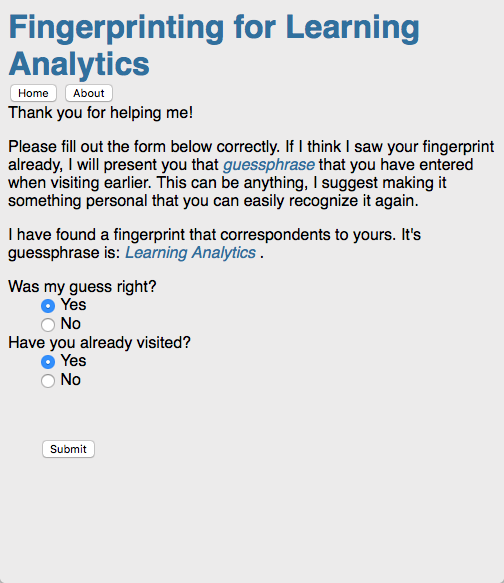
\includegraphics[height=3in]{img/fphp_secondvisit.png}}
\caption{Screenshot from \texttt{laprint}}
\label{fig:fpscreen}
\end{wrapfigure}
In order to get a rough estimate, how well we are able to hit cases $1$ and $4$ we will need some way to tell if we recognized users correctly. In a real life scenario this might be hard, but in our test case we can use an identifying phrase which we will call a \emph{guessphrase}. New users will be asked to provide such a identifying \emph{guessphrase} (e.g. name of first cat) which we will save together with the fingerprint. Revisiting users will be presented their \emph{guessphrase} and should tell, which of the above cases apply to them. This will of course be limited to a device and browser combination, since we are aiming for \emph{browser fingerprints} as explained in section \ref{sec:sota}. 

\subsection{Fingerprint creation}
\label{subsec:fingerprintvals}

We will limit our fingerprint to the basic \texttt{HTML} focused features. These should provide enough information to differentiate the small set of users. This will also facilitate the analysis, because we will only need to compare strings of features. Comparing different renderings in \texttt{WebGL} would introduce significant overhead in the sample implementation, whilst the main goal is to test recall and precision of the technique.

In Figure \ref{met:fig:headers} you can find all \texttt{HTTP-header} attributes we have collected from visiting users, together with values from one example visitor.


This recognition test, to again emphasize, aims to create a \textit{browser fingerprint}, not a \textit{device fingerprint}. In order to form the latter, additional feature extracted from the underlying hardware would be needed, which goes beyond the extent of this work. Cao and colleagues have already pointed out possibilities for doing so \cite{cao_cross-browser_2017}.

To test recall and precision for the fingerprints described in subsection \ref{subsec:userrecognition},we created a web service called \emph{Fingerprinting for Learning Analytics} which we used to fingerprint incoming users.\footnote{Inspired by the work of \href{amiunique.org}{amiunique}, but more lightweight.} It works roughly as follows:
\begin{wrapfigure}{l}{0.5\textwidth}
\centering
\footnotesize
\begin{tabular}{|p{2cm}|p{3cm}|}
\hline
	\texttt{HTTP-header} attribute & example \\ \hline\hline
	\texttt{user-agent} & Mozilla/5.0 (Macintosh; Intel Mac OS X 10.11; rv:58.0) Gecko/20100101 Firefox/58.0\\\hline
	\texttt{accept\-language} & de,en-US;q=0.7,en;q=0.3 \\\hline
	\texttt{accept\-encoding} & gzip, deflate \\\hline
	\texttt{accept} & text/html, application/xhtml+xml, application/xml; q=0.9, */*; q=0.8 \\ \hline
\end{tabular}
\caption{Collected \texttt{HTTP-header} values.}
\label{met:fig:headers}
\vspace{-1in}
\end{wrapfigure}



\begin{itemize}
	\item (1) Ask an incoming user, if she/he agrees on saving fingerprinting features of her/his browser.
	\item (2) Create a fingerprint and associating it with the user's \emph{guessphrase}.
	\item (2a) In case the fingerprint was recognized, the \emph{guessphrase} was presented and the user was asked whether it's correct.
	\item (3) Save the result for later analysis.
\end{itemize}

This is implemented rather straightforward. If the user agrees, we collect the \texttt{HTTP-Header} Attributes seen in Figure \ref{met:fig:headers} from the \texttt{request} object that is being sent with every \texttt{HTTP}-request. The 4-tuple \texttt{$($User-Agent$,$ Accept$,$ Accept-Language$,$ Accept-Encoding$)$} constructs the fingerprint $f_U$. We query our database for $f_U$ to see if the User is known. If we have seen $f_U$ in connection with multiple \emph{guessphrases}, we chose one of them at random and present them to the user. We could also have thrown an error, but in a real life scenario we wouldn't want to interrupt the users experience. Another solution would have been to then fall back to a default user. 

\pagebreak
\subsection{xAPI integration}

\begin{wrapfigure}{l}{0.55\linewidth}
\centering
\tiny
\begin{verbatim}
{
  "id":"12345678",
  "actor":{
    "openid":"http://www.example.org/video1/fp?acceptEncoding=gzip
      ,deflate\&UserAgent=Mozilla/5.0(Macintosh;IntelMacOSX10.11;.."
  },
  "verb":{
    "id":"http://adlnet.gov/expapi/verbs/watched",
    "display":{
      "en-US":"watched"
    }
  },
  "object":{
    "id:":"http://example.adlnet.gov/xapi/example/activity"
  }
}
\end{verbatim}
\caption{Sample xAPI Statement with Fingerprint (modified from documentation)}
\label{fig:xapi}
\end{wrapfigure}

Another subject to touch on is the integration with other Educational Technology. To properly use fingerprinting for tracking educational experiences, we need to have these fingerprints conform to a standard. A standardized exchange format is \texttt{xAPI}\footnote{Specification available on GitHub: \href{https://github.com/adlnet/xAPI-Spec}{xAPI-Spec}.}. Since a fingerprint in general will refer to a user that visits a website, we will propose ways to construct an \texttt{actor} object, that can then be combined with other properties to form a statement. The triple of (\texttt{actor}, \texttt{verb}, \texttt{object}) is minimal. Note that it will be impossible to come up with a fully standard compliant way to implement a fingerprint as an \texttt{actor} object, since these are required to only identify one agent or a group of agents, which cannot be guaranteed by fingerprinting.

The first way to construct the \texttt{actor} object which would be most intuitive, is to simply store all fingerprint attributes. This would result in a user object that is similar to what the fingerprinting entity has seen, adding no further complication.
Unfortunately, the xAPI specification forbids an \texttt{actor} object to be customized and only allows it to have one out of four Inverse Functional Identifiers from which we can already exclude \texttt{mbox}, \texttt{mbox\_sha1sum} and \texttt{account}. If these could be obtain or created, fingerprinting would possibly be obsolete. 

The only way to construct a valid IFI would be to create an OpenID. The URI would begin with the site that the fingerprinted user has visited and then store all attributes in a form of query attributes.\footnote{e.g.: \texttt{http://www.example.org/video1/fp?acceptEncoding=gzip,deflate\&User Agent=Mozilla/5.0(Macintosh;IntelMacOSX10.11;}[...]} We would then have encapsulated the fingerprint in the \texttt{actor} object to build a statement with, as seen in Figure \ref{fig:xapi}.

% section introduction (end)
% !TEX root = ../main.tex
\section{Results} % (fold)
\label{sec:results}


\begin{wrapfigure}{r}{0.4\linewidth}
\centering
\begin{tabular}{|r|c|}
\hline
Total Fingerprints & $34$ \\ \hline
Valid Fingerprints & $32$ \\ \hline
Unique Fingerprints & $26$\\ \hline
\end{tabular}
\caption{Descriptives}
\label{fig:fpstats}
\vspace{-0.25in}
\end{wrapfigure}


We ran the site from March 14. until March 19, mostly visited by friends and colleagues, see Figure \ref{fig:fpstats} for general metrics. We excluded $2$ of the total $34$ collected fingerprints because they did not have a \emph{guessphrase} associated. Thus we cannot decide whether they stem from the same browser or different ones. We see on first glance that roughly $\frac{3}{4}$ of incoming devices where in an anonymity set of size $1$ only by collecting the \texttt{HTTP-Header}. It must be noted that it's likely that this fraction rapidly drops for larger $N$, as Laperdrix and colleagues found it to only directly identify $\frac{3}{4}$ of visiting devices \cite{laperdrix_beauty_2016}. Similar to their findings, the \texttt{User-Agent} attribute adds the most diversity to the fingerprint, which can be seen in Figure \ref{res:fig:headers}.

\begin{wrapfigure}{l}{0.4\textwidth}
\centering
\footnotesize
\begin{tabular}{|p{2cm}|p{1cm}|}
\hline
\texttt{HTTP-header} attribute & unique values \\ \hline\hline
\texttt{user-agent} & $24$ \\\hline
\texttt{accept} & $5$ \\ \hline 
\texttt{accept encoding} & $1$ \\\hline
\texttt{accept language} & $10$ \\\hline
\end{tabular}
\caption{Fingerprints}
\label{res:fig:headers}
\end{wrapfigure}
The fingerprinting service we ran also asked visiting users for giving a \emph{guessphrase} that we associated with their fingerprint. This was inteded to make the service more engaging. Furthermore we encouraged them to revisit in order to find out, whether their fingerprint has changed. Finally this enabled us to have a look at precision and recall. Surprisingly despite only $75\%$ of fingerprints being unique, both recall and precision were either $1$ or rather close to $1$, see Figure \ref{fig:precrec}. 

While being seemingly good news at first, it also seems rather unlikely, having only $\frac{3}{4}$ of unique fingerprints. Since one user personally reported that they already saw a \emph{guessphrase} when visiting for the first time with a browser, we assume that users did not fill out the form completely if the \emph{guessphrase} did not match. Unfortunately, we did not track this case when running the site. 
\begin{wrapfigure}{r}{0.4\linewidth}
\centering
\begin{tabular}{|c|c|c|}
\hline
Metric & Value \\ \hline
Total & $79$\\\hline
True Positive & $46$\\\hline
False Positive & $2$\\\hline
True Negative & $31$\\ \hline
False Negative & $0$\\\hline \hline 
Precision & $0.95$ \\ \hline
Recall & $1.00$\\\hline
\end{tabular}
\caption{Precision \& Recall}
\label{fig:precrec}
\vspace{-0.25in}
\end{wrapfigure}
In order to test the validity of our results, we ran a test in which we tried to guess the \emph{guessphrase} of the fingerprints we had already collected. This gave us a value of $0.81$ for precision, which seems more reasonable. Unfortunately we couldn't retrieve recall from the simulation since constructing negatives by splitting our dataset would have decreased the number of fingerprints too much to still make reasonable statements about them.

After our test had ended, multiple users reported via mail, that the script was completely unable to recognize their devices. After looking at the corresponding fingerprints, we saw that they indeed were unique. This occurred with two Samsung smartphones, which suggests the frontend part of our tool was faulty and did not change the display accordingly. 
% !TEX root = ../main.tex
\section{Conclusion} % (fold)
\label{sec:conclusion}

In this paper we assessed the recent research on fingerprinting and tested some of the techniques with the help a web service. As discriminating as the technique has been shown to be, there must be cases where it is not. Especially institutions that issue a large number of identically configured devices that are running the exact same OS configurations and possibly are updated centrally altogether, will create one or a small number of anonymity sets. Thus, fingerprinting likely will not replace previous ways of identifying users like cookies or log-ins. Despite these limitations, it can prove to be a valuable addition to other identification techniques. In our use case, fingerprinting could potentially be a initial identification technique that can personalize content for a new visiting user until he decides to \textit{upgrade} to a standard user account. Also, when improving recommendation systems, the number of associated visitors of some educational material might be small or diverse enough for fingerprinting to be sufficient to uniquely identify the set of visitors. 

% section introduction (end)
\pagebreak
\section{References}
\label{sec:References}

\bibliographystyle{ieeetr}
\bibliography{LA_bibl.bib}
\pagebreak
% !TEX root = ../main.tex
\appendix

\section{Tables}
\label{fptable}

\begin{table}[!h]
\centering
\footnotesize
\begin{tabular}{|p{3.5cm}|p{2cm}|p{2cm}|p{3cm}|c|}
Attribute-Name & Source & Remark & Example Value & Studies\\ \hline \hline
\texttt{User-Agent} & \texttt{HTTP-Header} & &Mozilla/5.0 (Macintosh; Intel Mac OS X 10.11; rv:58.0) Gecko/20100101 Firefox/58.0 & \cite{laperdrix_beauty_2016,eckersley_how_2010} \\\hline
\texttt{accept} & \texttt{HTTP-Header} &  & text/html, application/xhtml+xml, application/xml; q=0.9, */*; q=0.8 & \cite{laperdrix_beauty_2016,eckersley_how_2010}\\\hline
\texttt{accept-encoding} & \texttt{HTTP-Header} & & gzip, deflate & \cite{laperdrix_beauty_2016,eckersley_how_2010} \\\hline
\texttt{accept-language} &\texttt{HTTP-Header} & &de,en-US;q=0.7,en;q=0.3 & \cite{laperdrix_beauty_2016,eckersley_how_2010} \\ \hline
List of HTTP-Headers & \texttt{HTTP-Header} & & see above & \cite{laperdrix_beauty_2016} \\\hline
List of Fonts & \texttt{Flash}, \texttt{Java}, \texttt{JavaScript} & & Abyssinica SIL, Aharoni CLM, AR PL UMing CN, $\ldots$ \cite{laperdrix_beauty_2016} & \cite{laperdrix_beauty_2016} \\\hline
List of plug-ins & \texttt{JavaScript} & & Plugin 1: Chrome PDF Viewer, Plugin 2: $\ldots$ \cite{laperdrix_beauty_2016} & \cite{laperdrix_beauty_2016} \\ \hline
\texttt{Timezone} & \texttt{JavaScript} & & -60 (UTC+1) \cite{laperdrix_beauty_2016} & \cite{laperdrix_beauty_2016} \\\hline
Screen Resolution \& Color Depth & \texttt{JavaScript} & & 1920x1200x24 \cite{laperdrix_beauty_2016} & \cite{laperdrix_beauty_2016,acar_fpdetective_2013}\\ \hline
Cookies enabled & \texttt{JavaScript} & & yes \cite{laperdrix_beauty_2016} & \cite{laperdrix_beauty_2016} \\\hline
Use of local/session storage & \texttt{JavaScript} & & yes \cite{laperdrix_beauty_2016} & \cite{laperdrix_beauty_2016} \\\hline
\texttt{navigator.platform} & \texttt{JavaScript} & spoofed \texttt{User-Agent}& MacIntel & \cite{laperdrix_beauty_2016,acar_fpdetective_2013} \\ \hline
\texttt{WebGL Renderer} & \texttt{JavaScript} & & NVIDIA Corporation \cite{laperdrix_beauty_2016} & \cite{laperdrix_beauty_2016,mowery_pixel_2012} \\\hline
\texttt{WebGL Vendor} & \texttt{JavaScript} & & GeForce GTX 650 \cite{laperdrix_beauty_2016} & \cite{laperdrix_beauty_2016,mowery_pixel_2012} \\\hline
Do Not Track Flag & \texttt{JavaScript} & & yes & \cite{laperdrix_beauty_2016} \\\hline
HTML5-canvas & \texttt{JavaScript} & & & \cite{laperdrix_beauty_2016,mowery_pixel_2012} \\\hline
Usage of an AdBlocker & \texttt{JavaScript} & & no \cite{laperdrix_beauty_2016} & \cite{laperdrix_beauty_2016} \\\hline
IP Address & IP Layer & Mostly for respawning & \texttt{127.0.0.1} & \cite{yen_host_2012} \\\hline
Browser Vendor \& Version & Feature availability & & Firefox/58.0 & \cite{nikiforakis_cookieless_2013} \\ \hline
\end{tabular}
\caption{Recently studied browser attributes}
\end{table}

\end{document}